\documentclass[preprint]{elsarticle}

\usepackage{amsmath}
\usepackage{amsfonts} %potrzebne do \mathbb{S}

\usepackage{here}

\usepackage{graphicx}
\usepackage{caption}
\usepackage{subcaption}

\usepackage{color}

\def\spe{\mathbf{Spec}}

\usepackage{graphicx}

\usepackage{soul}           %package for highlight
\newcommand{\noop}[1]{}

\usepackage{epstopdf}
% \usepackage{lineno,hyperref}
% \modulolinenumbers[5]

\journal{Applied Acoustics}

%%%%%%%%%%%%%%%%%%%%%%%
%% Elsevier bibliography styles
%%%%%%%%%%%%%%%%%%%%%%%
%% To change the style, put a % in front of the second line of the current style and
%% remove the % from the second line of the style you would like to use.
%%%%%%%%%%%%%%%%%%%%%%%

%% Numbered
%\bibliographystyle{model1-num-names}

%% Numbered without titles
%\bibliographystyle{model1a-num-names}

%% Harvard
%\bibliographystyle{model2-names.bst}\biboptions{authoryear}

%% Vancouver numbered
%\usepackage{numcompress}\bibliographystyle{model3-num-names}

%% Vancouver name/year
%\usepackage{numcompress}\bibliographystyle{model4-names}\biboptions{authoryear}

%% APA style
%\bibliographystyle{model5-names}\biboptions{authoryear}

%% AMA style
%\usepackage{numcompress}\bibliographystyle{model6-num-names}

%% `Elsevier LaTeX' style
%\bibliographystyle{abbrvnat}\biboptions{sort&compress}
\bibliographystyle{elsarticle-num}
%%%%%%%%%%%%%%%%%%%%%%%

\begin{document}

\begin{frontmatter}

\title{Application of cointegration to vibration signal for local damage detection in gearboxes}


%% Group authors per affiliation:
\author[label1]{Anna Michalak}
\author[label2]{Jacek Wodecki}
\author[label1]{Agnieszka Wy{\l}oma{\'n}ska}
\author[label2]{Radoslaw Zimroz}


\address[label1]{Research and Development Centre, KGHM Cuprum Ltd, Sikorskiego 2-8, 53-659 Wroclaw, Poland
\\ \{amichalak, awylomanska\}@cuprum.wroc.pl\\}

\address[label2]{Diagnostics and Vibro-Acoustic Science Laboratory, Wroclaw University of Science and Technology, Na Grobli 15, 50-421 Wroclaw
\\\{jacek.wodecki, radoslaw.zimroz\}@pwr.edu.pl\\}

\begin{abstract}
The problem of local damage detection for rotating machines is widely studied in the literature. In order to extract the information of the damage, the approach based on the vibration signal analysis is usually applied. Very often classical methods suited for impulsiveness analysis are not sufficient, therefore it is proposed to analyze the signal in terms of its periodicity features. In this paper the cointegration approach is  applied to vibration signal in the context of local damage detection in gearbox. The goal of this approach is to recognize if the examined signal comes from healthy or damaged machine. Firstly, we assume periodic correlation of given signal and measure its period. Afterwards, signal is restructured and divided into sub-signals according to the discovered period. Finally, we check if sub-signals are integrated and calculate the cointegrating vector by using the least squares method. In the paper we present details of the method and benefits of using our procedure. To validate our methodology we used simulated vibration signal based on typical gearbox used in mining industry, as well as real data from the gearbox. In the paper authors present a concept of the complete procedure that uses cointegration interpretation as a diagnostic measure.
\par

In this paper authors discuss the problem of fault detection in rotating machines. It is proposed to applied cointegration approach to vibration signal for detect local damage. It is based on the assumption of periodic correlation in the input signal. Data is restructured according to discovered period, and obtained subsignals are tested for integration and the cointegrating vector is calculated by using the least squares method. Finally, distances between non-zero elements of cointegrating vector are tested against randomness using Wald-Wolfowitz test. If vector is corrensponding to healthy machine, the test does not reject the H0 hypothesis, otherwise the hypothesis is rejected.  Presented procedure is validated on simulated and real vibration signals coming from gearbox used in mining industry.
\end{abstract}

\begin{keyword}
periodic correlation, local damage detection, cointegration, vibration signal
\end{keyword}

\end{frontmatter}

% \linenumbers

\section{Introduction}

The issue of fault detection in rotating machines has been a challenging problem for many years. In the literature one can find many methods for damage detection in gears and bearings \cite{feng2013recent,randall2011rolling,samuel2005review,obuchowski2014recent}. In such class of machine elements, local damage produces cyclic impulses occurring in the vibration signal. Very often typical time series analysis is insufficient since impulses are usually hidden in background noise or other low-frequency components related to normal operation of the machine \cite{wodecki2016combination,wodecki2017local,kruczek2017modified,zak2014novel,zak20161932,wylomanska2016impulsive,makowski2014new,wylomanska2016application}. To deal with such conditions, researchers often look for other domains, e.g. time-frequency domain. Unfortunately sometimes it is not helpful either.

In presented paper authors propose to use cointegration analysis to identify impulsive behavior present in vibration signal. Cointegration is a statistical property of a set of time series variables, that is very important in time series analysis, and is connected to stochastic trend analysis. It is widely used in the fields of finance and econometrics, and recently also for structural health monitoring (SHM) \cite{shi2016nonlinear,cross2011cointegration}. In the simplest words, we say that two processes X and Y are cointegrated, when neither of them hovers around a constant value or deterministic trend, but some linear combination of them does, so we can think of cointegration as a feature of long-term equilibrium relationship. The most visual examples of cointegrated processes are: income and consumption, or size of police force and amount of criminal activity. In this application, set of variables is realized by constructing specific array of subsignals based on original vibration signal. 

It is important to explain the reasons of this approach. Typically when analyzing periodically correlated data, one would calculate two-dimensional sample coherence map that provides a lot of information about signal periodicity. In presented case dataset is too big, which makes calculating such map not only too long in terms of execution time, but practically impossible in terms of memory utilization. Facing those limitations, authors decided to determine appropriate periodicity information based on one-dimensional coherence, that for used dataset can be calculated quickly, and use it to perform cointegration analysis.

\section{Methodology}

\textcolor{red}{We assume the considered vibration signal is periodically correlated (PC). The PC time series in engineering sciences is called cyclostationary. }PC property of given signal could be related to the fault in the machine but also to time-varying load condition or other cyclic modulation phenomena. In complex machines such as multistage gearbox it could be related to interaction between components. We remind the reader, that PC time series has periodic mean and the autocovariance functions with the same period $T$ \cite{hurd2007periodically}. If $\{X(n)\}$, $n=1,2,..,N$ is a second order PC time series, then two conditions are satisfied:

\begin{equation}
\label{eq:PC.process}
\begin{gathered}
m_X(n)=E\left(X(n)\right)=m_x(n+T) \\
R_X(n,m)=E(X(n)-m_X(n)(X(m)-m_X(u))=R_X(n+T,m+T)
\end{gathered}
\end{equation}

\textcolor{red}{There are different methods that can be used to period $T$ recognition, see for instance \cite{antoni2004cyclostationary}. In this paper we propose to apply  the coherent statistic \cite{hurd2007periodically} (CS) which is defined as follows:}

\begin{equation}
\label{eq:coherence}
\begin{gathered}
|\gamma(\omega_p,\omega_q,M)|^2=\frac{|\sum_{m=0}^{M-1}I_N(\omega_{p+m})\overline{I_N(\omega_{q+m})} |^2}{\sum_{m=0}^{M-1}|I_N(\omega_{p+m})|^2\sum_{m=0}^{M-1}|I_N(\omega_{q+m})|^2},
\end{gathered}
\end{equation}
where $I_N(\omega)=\sum_{n=1}^{N}X(n)e^{-i \omega(n-1)}$ in point $\omega_k=\frac{2 \pi(k-1)}{N}$, $k=1,2,\dots,N$. On the basis of CS one can calculate one dimensional coherence $|\gamma(0,\omega_d,N-d)|^2$ which takes values between $[0,1]$. If on the CS plot one can observe peaks in points $(\omega_d,2\omega_d,3\omega_d,\dots)$ then the period $T$ is recognized as $T=\frac{1}{\omega_d}$. This is the period that is used later on. 

It is worth to mention, the PC time series are very popular in different applications, see for instance \cite{antoni2004cyclostationary,broszkiewicz2004detecting}.

As it is proved in \cite{broszkiewiczperiodic} there is a strong relation between PC time series and so-called intergrated and cointegrated ones. First we remind the reader the definitions of integration and cointegration. 

We say the given time series $\{X(n)\}$ is integrated with order $d$, if the increments of the time series $\left(\Delta X(n)=X(n)-X(n-1)\right)$ calculated $d$ times give the stationary time series. In this case we take the notation $X(n) \sim I(d)$.

We say the $m$ time series $\{X(1,n)\},…,\{X(m,n)\}$ are cointegrated with orders $d$ and $b$ if two conditions are satisfied:
\begin{enumerate}
\item The separate time series are integrated with order $d$.
\item 	There is a linear combination of the time series $\{X(1,n)\},\dots,\{X(m,n)\}$ e.g. $a_1 X(1,n)+a_2 X(2,n)+ \dots+a_m X(m,n)$,  which is integrated with order $d-b$. In this case the time series are denoted as ${X(1,n)},\dots,{X(m,n)}\sim CI(d,b)$. The vector $[a_1,\dots,a_m]$ is called the cointegrating vector. In practice, the  cointegrating vector is estimated from the real time series by using the least squares method.
\end{enumerate}

The concept of cointegration was introduced by Engle \cite{engle1987co} and first was applied in the financial data modeling. However in the last years one can find different interesting applications of the cointegration-based methodology \cite{tabrizi2016cointegration,worden2014multiresolution}. \textcolor{red}{In general, one can say that two or more time series are cointegrated if they are in some sense associated, they have the same pattern. In other words, they are correlated in mathematical sense. We remind the correlation (Pearson correlation) between two data sets means there is a linear dependence between them. }

According to the methodology applied in \cite{broszkiewiczperiodic} if the time series is PC, then  the appropriate selected sub-signals are integrated, moreover those sub-signals are also cointegrated. 
If the time series $\{X(n)\}$ is PC with period $T$, then the time series defined as follows:
\begin{equation}
\label{eq:subsignals}
\begin{gathered}
Y(v,n)=X(nT+v), \quad v=1,2,\dots,T
\end{gathered}
\end{equation}
are cointegrated with some appropriate order. The idea of calculating of $\{Y(v,n)\}$ time series from the raw signal is presented in Fig. \ref{fig:subsignals_scheme}.

\begin{figure}[ht!]
\centering
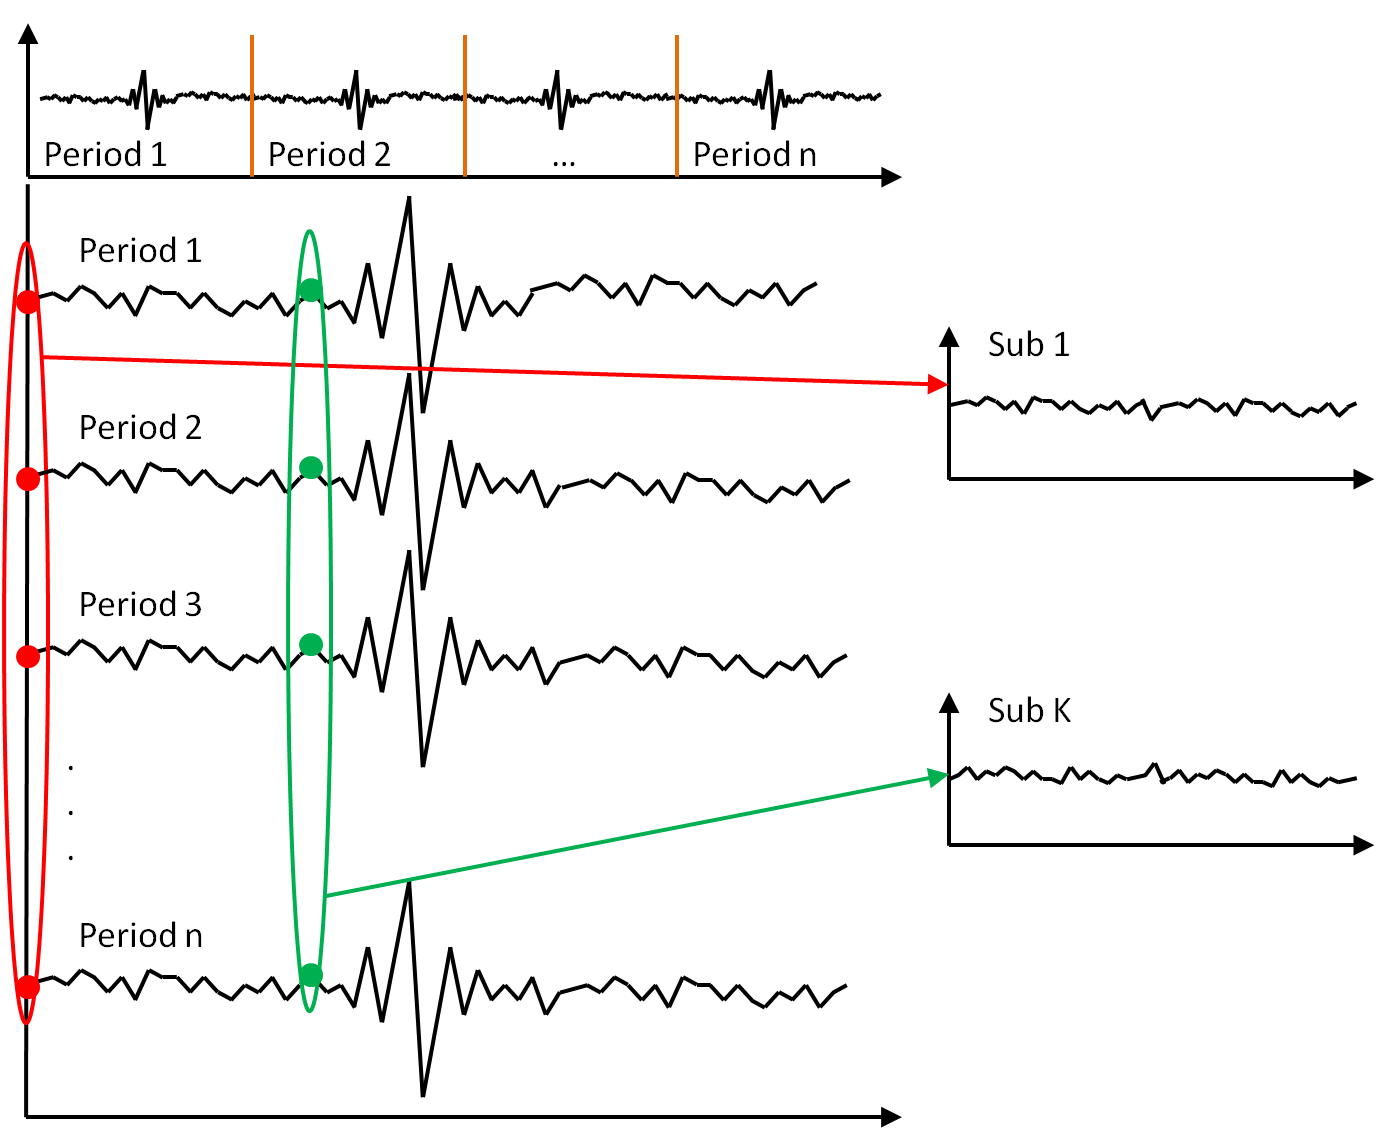
\includegraphics[width=0.48\textwidth]{wykresy/subsignals_scheme}
\caption{General idea of subsignals construction procedure.}
\label{fig:subsignals_scheme}
\end{figure}
The methodology applied in this paper was used in \cite{broszkiewiczperiodic} in the analysis of daily data from the power market. It was shown that analyzed time series exhibit PC-like behavior and on this basis the integration and cointegration was proved.\textcolor{red}{ There are many statistics which can be used to prove if given time series is integrated \cite{dickey1979distribution,kwiatkowski1992testing}. In this paper we propose to take under consideration Durbin-Watson statistic which for time series $\{X(n)\}$ is defined  as follows \cite{broszkiewiczperiodic}:
\begin{equation}
\label{eq:IDW}
\begin{gathered}
IDW=\frac{\sum\left(X(n)-X(n-1)\right)^2}{\sum\left(X(n)-\overline{X}(n)\right)^2},
\end{gathered}
\end{equation}
where $\overline{X}(n)$ is the sample mean of given time series.The Durbin-Watson statistic is always between 0 and 4. By using the $IDW$ statistic the  Durbin-Watson statistical test is constructed in order to detect the presence of autocorrelation (a linear relationship between the observations) of given time series. In the Durbin-Watson test the $H_0$ and alternative hypotheses are defined as:
\[H_0:~\rho=0\]
\[H_1:~\rho>0,\]
where $\rho$ is a first order autocorrelation, i.e. autocorrelation for lag equal to $1$.  The Durbin-Watson test is also considered as the appriopriate one applied to testing so-called unit root property (called also integration of order 1). On the basis of the upper ($d_U$) and lover ($d_L$) critical values of the test for given confidence level  one can reject or accept the $H_0$ hypothesis. More precisely:\\
If $IDW<d_L$, then $H_0$ hypothesis is rejected on given confidence level, i.e. there is  a first order autocorrelation between the time series and it is not stationary.\\
If $IDW>d_U$, then the $H_0$ hypothesis can not be rejected on given confidence level, i.e. the is no aucorrelation and the time series is stationary.\\
If $d_L<IDW<d_U$, test is inconclusive.\\
The critical values $d_L$ and $d_U$ one can find in the table of critical values of Durbin-Watson statistic.
In practice for number of observations a value of $IDW$ statistic close to $2$ means that there is no autocorrelation, i.e. the time series is stationary. Values approaching $0$ indicate positive autocorrelation and values toward $4$ indicate negative autocorrelation.}

In order to test if given time series is integrated  with order $d$ we propose to use the $IDW$ statistic as follows. First we calculate the $IDW$ statistic for raw time series, if the value of the statistic is close to $2$, then the time series is $I(0)$. If not, we take the increments and once again calculate the $IDW$ statistic for differenced time series. If $IDW \sim 2$, then the raw time series is $I(1)$, if not the we repeat the procedure as long as the $IDW$ statistic takes value close to $2$. 

After checking if appropriate time series are integrated with given order, we can check if they are cointegrated. First we should find the cointegrating vector $[a_1,\dots,a_m]$.\textcolor{red}{ As it was mentioned, the cointegrating vector is calculated by using least squares method in the multivariate regression model:
$$Y(1,n)=a_1 Y(2,n)-\dots -a_{(m-1)} Y(m,n).$$}
Next we calculate the residuals:

\begin{displaymath}
v(n)=Y(1,n)-a_1 Y(2,n)-\dots -a_{(m-1)} Y(m,n)
\end{displaymath}

Finally we check if they are integrated by using the $IDW$ statistic applied to $v(n)$.

In case of vibration data analysis first we assume PC behavior of the signal. Then we use the one dimensional coherence to obtain the main period. Next, we divide the signal into $T$ sub-signals according to presented methodology, see Fig. \ref{fig:subsignals_scheme}. Then we check if the sub-signals  are integrated and cointegrated by using the $IDW$ statistic. Finally, we present the cointegrating vector. It can be proven by using simulated and real signals  that the cointegrating vectors for the signal from healthy machine exhibits chaotic-like behavior, the components are not associated, while the cointegrating vector for damaged machine exhibits completely different behavior. We observe here the time stamps with larger values of the components of cointegrating vector. This corresponds to the division of the impulses related to damage in one cycle. The behavior is easy to explain. In case of the healthy machine, where the cyclic impulses do not occur, the appropriate sub-signals behave like a noise, they are not correlated, therefore the cointegrating vector is also random. If in the vibration signal the cyclic impulses related to damage occur, then the sub-signals containing those impulses are more associated with respect to sub-signals without impulses therefore in the cointegrating vector we observe the relationship between appropriate components. The schematic algorithm of the proposed procedure is presented in Fig. \ref{fig:algorytm}.

In order to test if the cointegrating vector corresponds to healthy or damaged machine we examine if it exhibits random (chaotic) behavior. In order to do this we apply the Wald-Wolfowitz test for randomness \cite{wald1940test} for distances between nonzero values of the vector $[a_1,a_2,\dots, a_n]$. If the cointegrating vector is related to healthy machine, the test does not reject the hypothesis of randomness ($H_0$) while in case of damaged machine $-$ the test reject the hypothesis (the $H_1$ is accepted). Here we analyze the corresponding \emph{p}-value and we reject the $H_0$ hypothesis if it takes small value (smaller than the confidence level $0.05$). The $H_0$ hypothesis is not rejected if the \emph{p}-value is greater than the confidence level.

\begin{figure}[ht!]
\centering

\includegraphics[width=0.38\textwidth]{wykresy/block_diagram.png}
\caption{Block diagram of the applied methodology.}
\label{fig:algorytm}
\end{figure}

\section{Simulated data}

In this section we examine the simulated data which  represents vibration signal from gearbox. Signal consists of the Gaussian noise and deterministic part given by four sine waves of 500, 1000, 1500 and 2000 Hz, acting as mesh components. They are frequency-modulated with modulation frequency 4 Hz. The damage frequency is equal to 8 Hz and the sampling frequency is 16384 Hz. Both signals (from healthy and damaged machine)  have 819200 observations, which translates into 50 seconds of data. Signal was generated according to the procedure described in \cite{wylomanska2014periodic}. In Fig. \ref{fig:simulated_signal_all} we observe simulated signal, and Fig. \ref{fig:simulated_signal_part} presents a short part of it for clear visibility. Time series presented on the top panels correspond with healthy gearbox and from the bottom panels describe the damaged one. As one can see the amplitude of faulty time series is much higher because of damage-related impulsive behavior. It is important to mention that impulses placed in simulated signal are characterized with high amplitude, which makes them clearly visible. Signal has been prepared this way just to allow for undisputed validation of the results.

\begin{figure}[ht!]
\centering
\includegraphics[width=0.48\textwidth]{wykresy/simulated_signal_all.eps}
\caption{Simulated signal corresponding to healthy (top panel) and damaged machine (bottom panel).}
\label{fig:simulated_signal_all}
\end{figure}

\begin{figure}[ht!]
\centering
\includegraphics[width=0.48\textwidth]{wykresy/simulated_signal_part.eps}
\caption{Short part of simulated signals presented for visibility.}
\label{fig:simulated_signal_part}
\end{figure}

Firstly we calculate one dimensional coherent statistic to recognize the period of the signal. In this statistic we observe major local maxima (Fig. \ref{fig:simulated_signal_coherence}). The distance between two peaks is 200 observations. If N is a length of the signal, then the period is T=N/200. In this case T=4096 observations, which gives 0.25 second.

\begin{figure}[ht!]
\centering
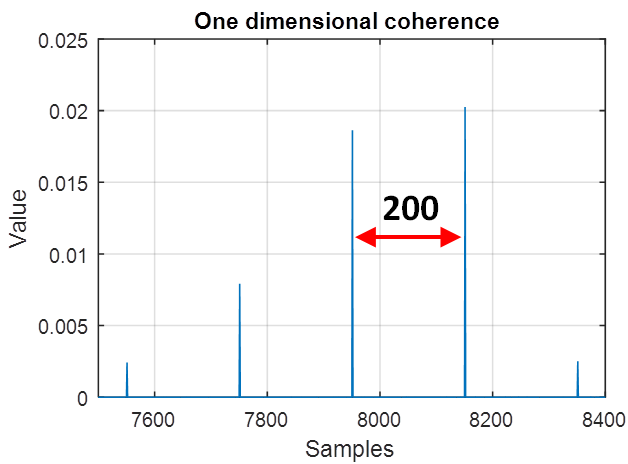
\includegraphics[width=0.48\textwidth]{wykresy/simulated_coherence.png}
\caption{One dimensionial coherence.}
\label{fig:simulated_signal_coherence}
\end{figure}

At this point the sub-signals are calculated. The number of sub-signals is the same as the period value of PC process, e.g. for period equal to 4096 we will obtain 4096 sub-signals. The exemplary sub-signals are presented in Fig. \ref{fig:simulated_subsignals}. On the top panel we observe the sub-signals related to the signal from healthy machine while the bottom panel shows sub-signals  coming from the damaged gearbox. The amplitude of the sub-signals from healthy machine  is clearly smaller than from the faulty one. 


\begin{figure}[ht!]
\centering
\includegraphics[width=0.48\textwidth]{wykresy/simulated_subsignals.eps}
\caption{The exemplary sub-signals extracted from healthy and damaged gearbox (simulated signal).}
\label{fig:simulated_subsignals}
\end{figure}

After extraction of appropriate sub-signals, first they are tested against the integration. In order to do this we calculate the Durbin-Watson statistic. In Fig. \ref{fig:simulated_IDW} we present the value of IDW statistic for all sub-signals. For both signals (from healthy and damaged machine) this statistic takes value close to two, so we can accept the hypothesis that  examined sub-signals are integrated I(0). \textcolor{red}{This confirms our assumption.}

\begin{figure}[ht!]
\centering
\includegraphics[width=0.48\textwidth]{wykresy/simulated_IDW.eps}
\caption{Durbin-Watson statistic for each of sub-signals from healthy (top panel) and damaged case (bottom panel)(simulated signal).}
\label{fig:simulated_IDW}
\end{figure}

	Next, by using the least squares method we calculate the cointegrating vector. In Fig. \ref{fig:simulated_vector_ok} we observe the part of the signal corresponding to one period (the first one) of healthy signal and corresponding cointegrating vector. The coefficients are distributed randomly, with Wald-Wolfowitz test accepting null hypothesis with \emph{p}-value equal to 0.2. Results indicate that the signal comes from the healthy gearbox.   

\begin{figure}[ht!]
\centering
\includegraphics[width=0.48\textwidth]{wykresy/simulated_vector_ok.eps}
\caption{The part of the signal (from healthy machine) corresponding to one  period (top panel) and cointegrating vector (bottom panel)(simulated signal).}
\label{fig:simulated_vector_ok}
\end{figure}

In Fig. \ref{fig:simulated_vector_damaged} we present the part of the signal corresponding to one period (the first one) for the faulty case. As we can see, there are two impulses in each period related to damage. The cointegrating vector is presented on the bottom panel. 

\begin{figure}[ht!]
\centering
\includegraphics[width=0.48\textwidth]{wykresy/simulated_vector_damaged.eps}
\caption{The part of the signal (from damaged machine) corresponding to one  period (top panel) and cointegrating vector (bottom panel)(simulated signal).}
\label{fig:simulated_vector_damaged}
\end{figure}

In this case it can be clearly seen that distribution of coefficients pattern changed significantly. One can notice two main groups that correspond to presence of impulses in the signal, with Wald-Wolfowitz test rejecting null hypothesis with \emph{p}-value equal to $3.6 \cdot 10^{-5}$. This indicates the signal corresponds to machine with local damage.

\section{Real data}

In this section we analyze two signals from the real life gearbox that is part of driving station for a belt conveyor operating in underground mining industry (Fig. \ref{fig:real_machine}). 

\begin{figure}[ht!]
\centering
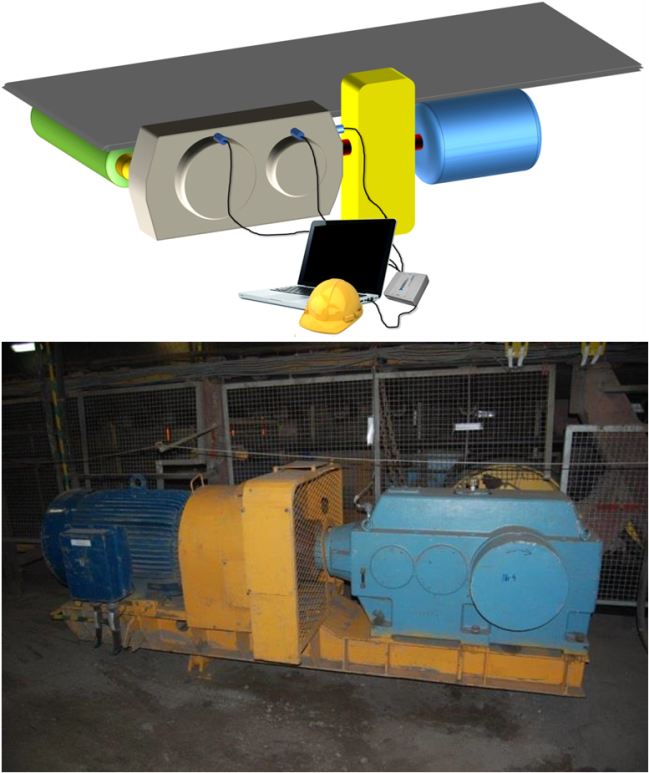
\includegraphics[width=0.48\textwidth]{wykresy/real_machine}
\caption{Example of two-stage gearbox operating in underground mine.}
\label{fig:real_machine}
\end{figure}

It is a two-stage gearbox with first stage being conical, and second – cylindrical. Simplified kinematic schematic of such gearbox is presented in Fig. 
\ref{fig:real_kinematic_scheme}.

\begin{figure}[ht!]
\centering
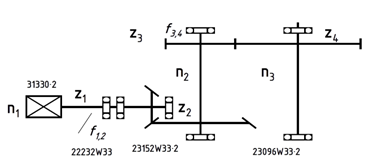
\includegraphics[width=0.48\textwidth]{wykresy/real_kinematic_scheme.png}
\caption{Simplified kinematic schematic of the gearbox}
\label{fig:real_kinematic_scheme}
\end{figure}

Frequency parameters of the gearbox are presented in Tab \ref{tab:mechanical_freq}

\begin{table}[]
    \centering
    \caption{Mechanical frequencies present in the gearbox}
    \resizebox{0.60 \textwidth}{!}{
    \begin{tabular}{|l|l|l|}
    \hline
        \textbf{Component} & \textbf{Frequency} & \textbf{Value} \\    \hline
        $f_{01}$ first shaft frequency & $f_{01}=\frac{n_1}{60}$ & 16.5 Hz \\
      $f_{02}$  second shaft frequency & $f_{01}=\frac{n_2}{60}=\frac{n_1}{60\cdot u_1}$&4.17 Hz \\
       $f_{03}$ third (output) shaft frequency& $f_{03}=\frac{n_3}{60}=\frac{n_1}{60\cdot u_1 \cdot u_2}$ & 1.18 Hz\\
       $f_{z1}$ meshing frequency of first stage & $f_{z1}=\frac{n_1 \cdot z_1}{60}$& 379.50 Hz\\
       $f_{z2}$ meshing frequency of second stage& $f_{z2}=\frac{n_2 \cdot z_2}{60}$ & 183.30 Hz \\
        $U_p$ Total gear ratio& $U_p =\frac{z2}{z1} \cdot \frac{z4}{z3}$ & 14,00 \\     \hline
    \end{tabular}
    }
    \label{tab:mechanical_freq}
\end{table}

The sampling frequency is 17066 Hz. Both signals have 1022676 observations, which translates to almost 60 seconds. Fig. \ref{fig:real_signal_all} shows raw vibration data for healthy and damaged gearbox, and again Fig. \ref{fig:real_signal_part} presents short part for visibility. The second signal comes from a year after the first one. Signal connected with damaged gearbox has a higher amplitude associated with impulse behavior of damages.

\begin{figure}[ht!]
\centering
\includegraphics[width=0.48\textwidth]{wykresy/real_signal_all.eps}
\caption{Raw vibration data from the gearbox from healthy (top panel) and damaged (bottom panel) machine (real signal).}
\label{fig:real_signal_all}
\end{figure}

\begin{figure}[ht!]
\centering
\includegraphics[width=0.48\textwidth]{wykresy/real_signal_part.eps}
\caption{Short part of real life signals presented for visibility (real signal).}
\label{fig:real_signal_part}
\end{figure}

Real data analysis utilizes the same procedure as applied for simulated signals, assuming PC properties. We observe peaks in one dimensionial coherence statistic calculated for both signals (Fig. \ref{fig:real_coherence} presents the statistic calculated for the damaged gearbox). The distance between peaks is 248 which gives us the period $T=\frac{1022676}{248}=4123$. 

\begin{figure}[ht!]
\centering
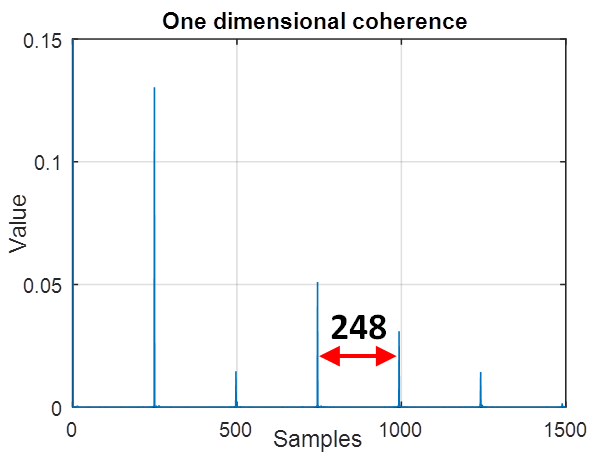
\includegraphics[width=0.48\textwidth]{wykresy/real_coherence.png}
\caption{One dimensional coherence.}
\label{fig:real_coherence}
\end{figure}

Calculated sub-signals are presented in Fig. \ref{fig:real_subsignals} for healthy (top panel) and damaged (bottom panel) machine. Behavior of sub-signals related to healthy machine is random, but in damaged case we can observe the presence of deterministic components, in this case data seem to be correlated.

\begin{figure}[ht!]
\centering
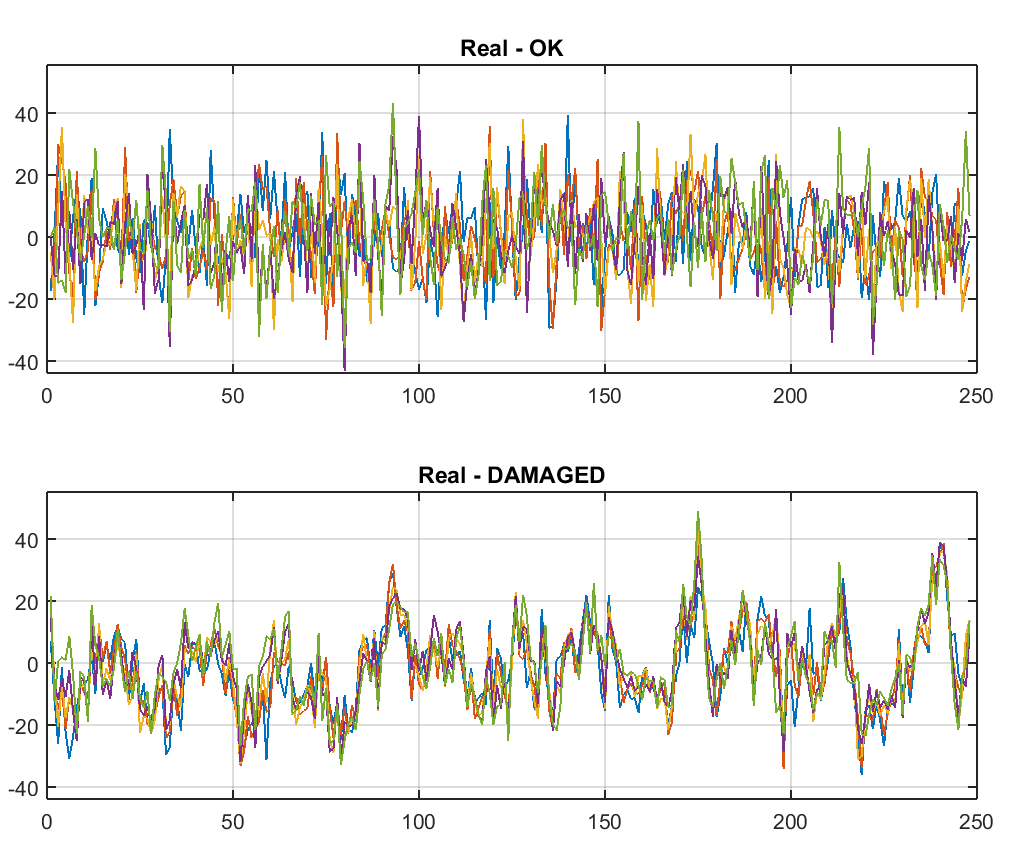
\includegraphics[width=0.48\textwidth]{wykresy/real_subsignals.png}
\caption{The exemplary sub-signals extracted from signal corresponding to healthy (top panel) and damaged (bottom panel) gearbox (real signal).}
\label{fig:real_subsignals}
\end{figure}

In order to prove that the sub-signals are integrated, we calculate Durbin-Watson statistic. In Fig. \ref{fig:real_IDW} we present the value of IDW statistic for each sub-signal. The blue color corresponds with IDW statistics for sub-signals (without differentiation), and the red one with IDW statistics after single differentiation. Sub-signals corresponding to healthy gearbox are integrated with order zero but those connected with damaged one are I(1).

\begin{figure}[ht!]
\centering
\includegraphics[width=0.48\textwidth]{wykresy/real_IDW.eps}
\caption{Durbin-Watson statistic for each of sub-signals from healthy (top panel) and damaged case (bottom panel) (real signal).}
\label{fig:real_IDW}
\end{figure}

By using the least squares method applied to multivariate linear regression model we estimate cointegrating vectors for both of examined  signals, i.e. from healthy and damaged machine. In Fig. \ref{fig:real_vector_ok} we present one part of the signal corresponding to one period from healthy gearbox and related cointegrating vector. As one can see, the coefficients for the healthy gearbox are spread randomly, with Wald-Wolfowitz test accepting null hypothesis with \emph{p}-value equal to 0.87. This suggests that signal does not contain any anomalies.

\begin{figure}[ht!]
\centering
\includegraphics[width=0.48\textwidth]{wykresy/real_vector_ok.eps}
\caption{The part of the signal (from healthy machine) corresponding to one  period (top panel) and cointegrating vector (bottom panel) (real signal).}
\label{fig:real_vector_ok}
\end{figure}

For the signal corresponding to the damaged gearbox two anomalies can be observed (Fig. \ref{fig:real_vector_damaged}). We can see that cointegrating vector concentrates into two groups, with Wald-Wolfowitz test rejecting null hypothesis with \emph{p}-value equal to $1.2 \cdot 10^{-21}$. 

\begin{figure}[ht!]
\centering
\includegraphics[width=0.48\textwidth]{wykresy/real_vector_damaged.eps}
\caption{The part of the signal (from damaged machine) corresponding to one  period (top panel) and cointegrating vector (bottom panel) (real signal).}
\label{fig:real_vector_damaged}
\end{figure}


\section{Conclusions}
In the presented paper we propose a new approach to local damage identification based on cointegration issue. We assume the analyzed vibration signal exhibits the cyclostationaty behavior and therefore the appropriate sub-signals are cointegrated. The cointegration here means the relationship between the vectors. The main point is the cointegrating vector analysis. We have proved for the vibration signal from healthy machine it exhibits chaotic-like behavior unlike for the damaged case. By application of the statistical test for randomness we can clearly detect if the cointegrating vector is related to the unhelathy machine. This approach extends the family of local damage detection methods based on the vibration signal analysis.  Methodology comprehensively covers the topics of practical implementation and use, quantification and interpretation of diagnostic features. Algorithm is verified against simulated and real-life industrial data. 

\section*{Acknowledgments}

The work is supported by the Framework Programme for Research and Innovation Horizon 2020 under grant agreement n. 636834 (DISIRE - Integrated Process Control based on Distributed In-Situ Sensors into Raw Material and Energy Feedstock).


\section*{References}

\bibliography{mybibfile}

\end{document}